\section{ICMP}
\subsection{NAT/PAT}
Da ICMP Pakete keine Ports kennen muss ein Router seine PAT Tabelle anders realisieren.
Er verwendet dazu die Sequenznummern der Echo/Reply Pakete. Die Sequenznummern dienen dazu eine Antwort einem Request zuzuweisen. Ein Implementationsvariante ist, dass der Router anstelle des Ports die Sequenznummer verwendet, oder diese einem virtuellen Port zuweist.

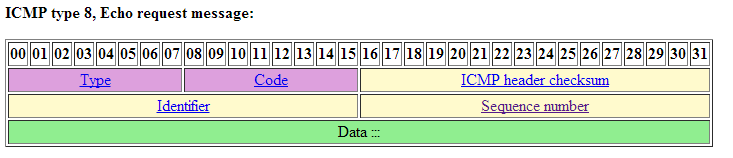
\includegraphics[scale=0.8]{media/ICMPRequest.png}

